\begin{figure}[htbp]
    \centering
    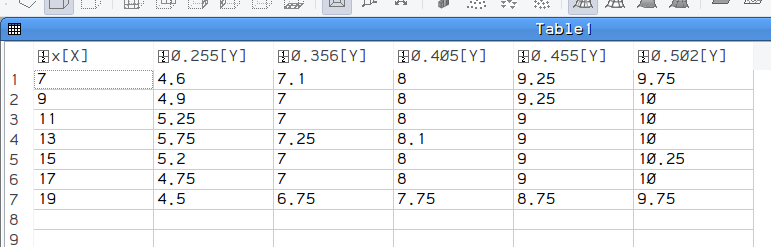
\includegraphics[width=0.35\textwidth]{reta/1dados.png}

    \caption{Dados de corrente por tensão, gerados por computador}
    \label{fig:reta:dados}
\end{figure}

Nesta seção, será tomado como exemplo a relação de corrente e tensão em um resistor, dado de forma teórica pela relação (\ref{eq:resist}). Por mais os dados usados aqui sejam os da figura \ref{fig:reta:dados}, essa parte de apresentação de dados é importante para todos tipo de análise, em especial, para dados coletados manualmente, como é o caso dos experimentos da disciplina de \texttt{F 329}.

\begin{equacao} \label{eq:resist}
    I = \frac{1}{R} ~ V
\end{equacao}


\subsection{Dados Pontuais}

    Normalmente, quando se trata de dados pontuais, é importante mostrar esses dados em alguma tabela e no gráfico também. O modo de se fazer isso no \software é com a funcionalidade \texttt{Scatter} (figura \ref{fig:reta:scatter}).

    \begin{figure}[htbp]
        \centering
        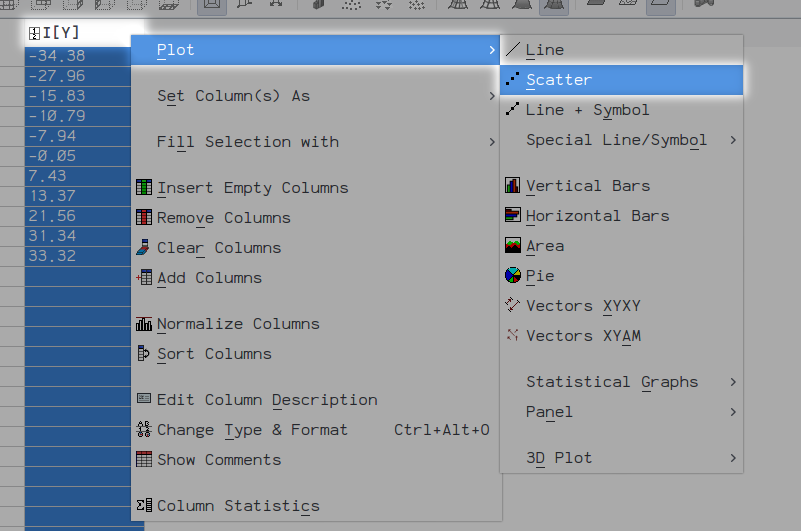
\includegraphics[width=0.6\textwidth]{reta/2scatter.png}

        \caption{\texttt{Scatter}}
        \label{fig:reta:scatter}
    \end{figure}

    \begin{figure}[htbp]
        \centering
        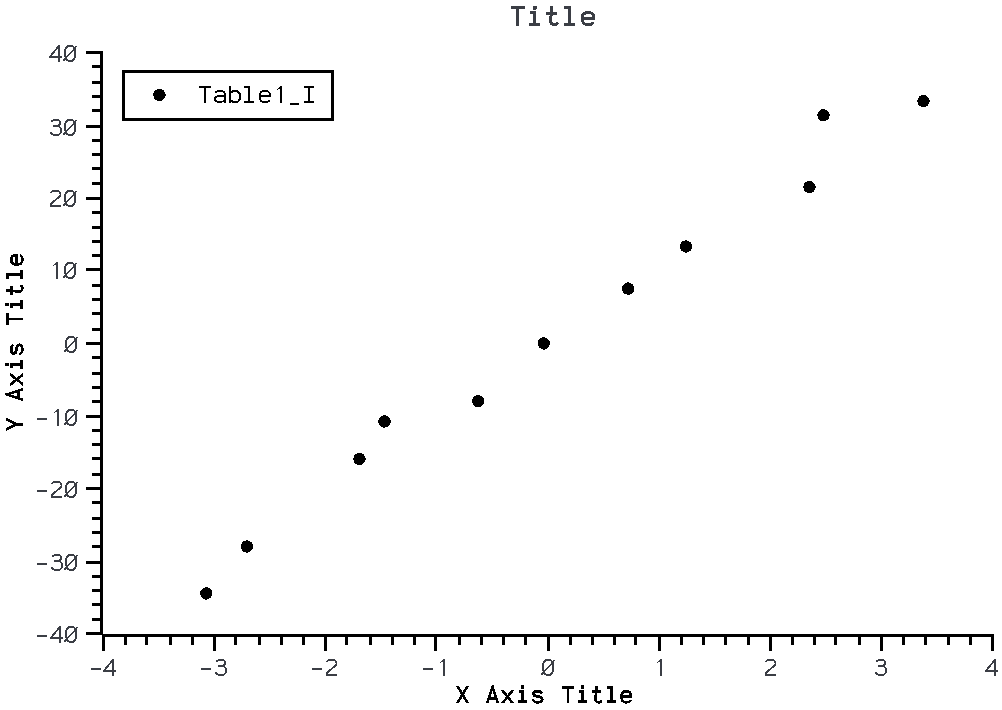
\includegraphics[width=0.5\textwidth]{reta/1linscatter.pdf}

        \caption{Resultado do \texttt{Scatter}}
        \label{fig:reta:linscatter}
    \end{figure}


\subsection{Tratamento da Legenda}

    O \software gera uma legenda padrão para os elementos desenhados no gráfico. O ideal é alterá-las para serem mais informativas. As legendas também podem ser reposicionadas apenas arrastando-as. Por padrão, o plano de fundo da legenda é transparente, mas é recomendável mudar para um plano de fundo preenchido em branco ou qualquer que seja a cor de fundo do gráfico.

    \begin{figure}[htbp]
        \centering
        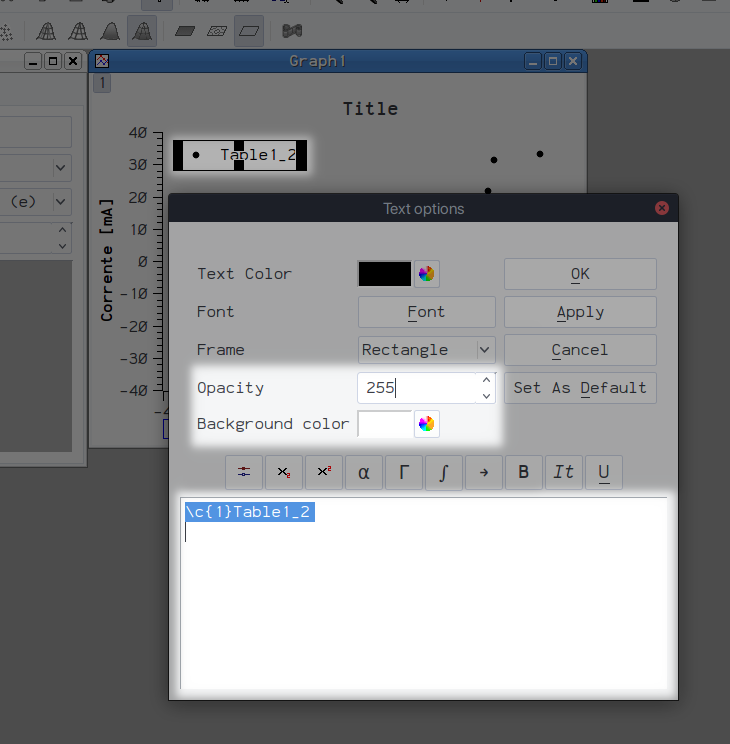
\includegraphics[width=0.5\textwidth]{reta/3legenda.png}

        \caption{Alterando o texto da legenda}
        \label{fig:reta:legenda}
    \end{figure}


\subsection{Formatação dos Eixo e do Título}

    Diferente do \texttt{Origin}, o \software não ajusta nada nos texto do gráfico, então isso deve ser feito manualmente, como é visto nas figuras \ref{fig:reta:eixo} e \ref{fig:reta:titulo}.

    \begin{figure}[htbp]
        \centering
        \begin{subfigure}{0.45\textwidth}
            \centering
            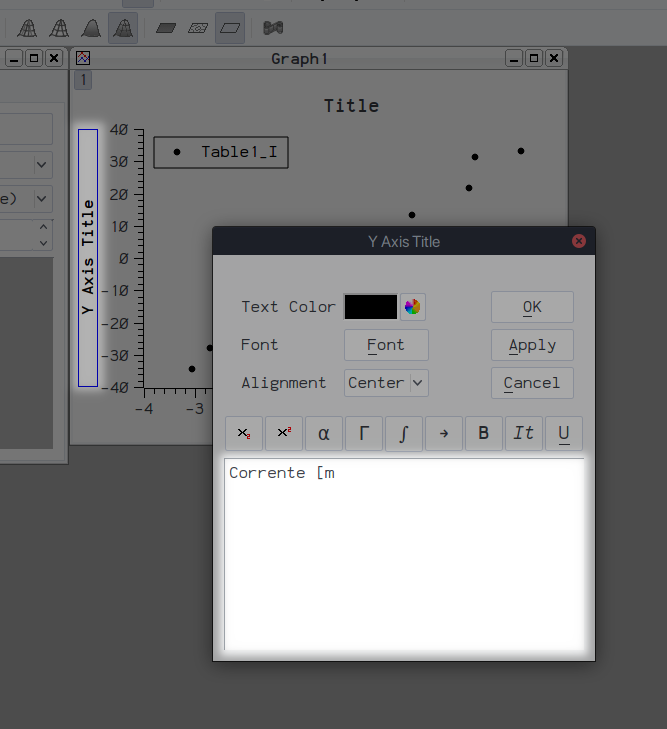
\includegraphics[width=\textwidth]{reta/4eixos.png}

            \caption{Alterando dos nomes dos eixos}
            \label{fig:reta:eixo}
        \end{subfigure}
        ~
        \begin{subfigure}{0.45\textwidth}
            \centering
            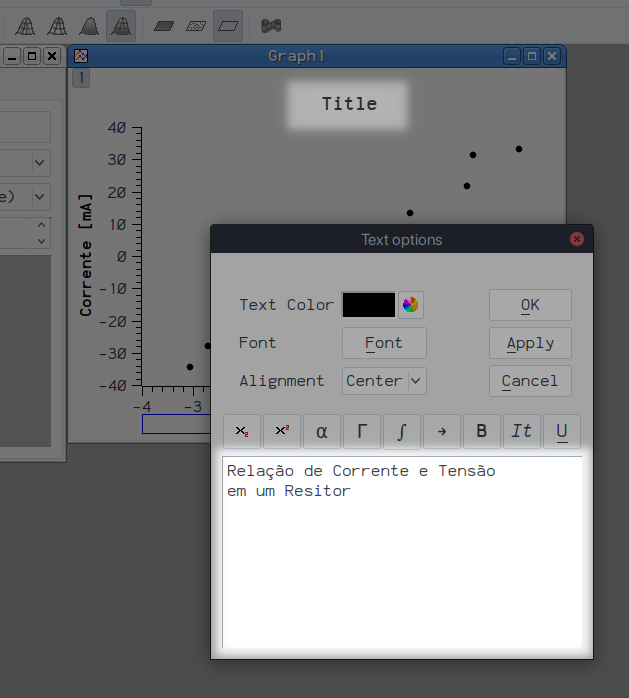
\includegraphics[width=\textwidth]{reta/4titulo.png}

            \caption{Mudança do título}
            \label{fig:reta:titulo}
        \end{subfigure}
        \caption{Opções dos textos principais do gráfico}
        \label{fig:reta:textos}
    \end{figure}


\subsection{Linhas de Grid}

    Para ler melhor os eixos do gráfico, é possível colocar linhas de \textit{grid} acompanhando os valores principais.

    \begin{figure}[htbp]
        \centering
        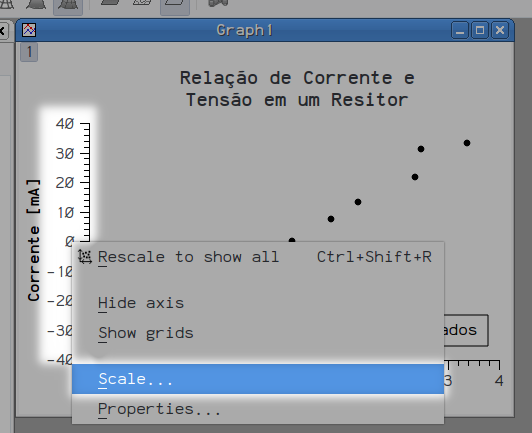
\includegraphics[width=0.55\textwidth]{reta/5gridopt.png}

        \caption{Acesso as opções de formatação de linha de acompanhamento dos eixos}
        \label{fig:reta:gridopt}
    \end{figure}

    No material, serão utilizadas linhas principais horizontais e verticais, que serão em tracejados em cinza escuro, sem linhas secundárias. Essas configurações podem e devem ser alteradas para cada gráfico, dependendo da e facilidade e da importância da leitura dos valores.

    \begin{figure}[htbp]
        \centering
        \begin{subfigure}{0.45\textwidth}
            \centering
            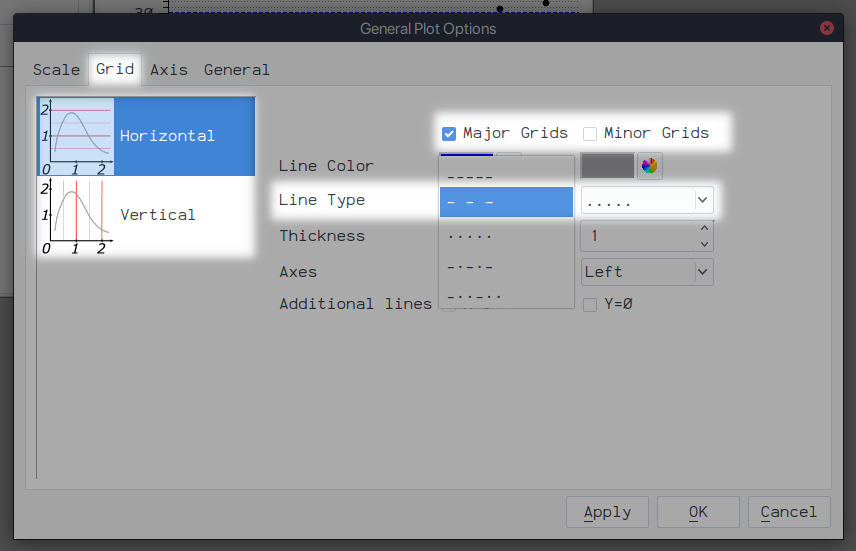
\includegraphics[width=\textwidth]{reta/6grid.png}

            \caption{Opções dos eixos (aba \texttt{Grid})}
            \label{fig:reta:grid}
        \end{subfigure}
        ~
        \begin{subfigure}{0.45\textwidth}
            \centering
            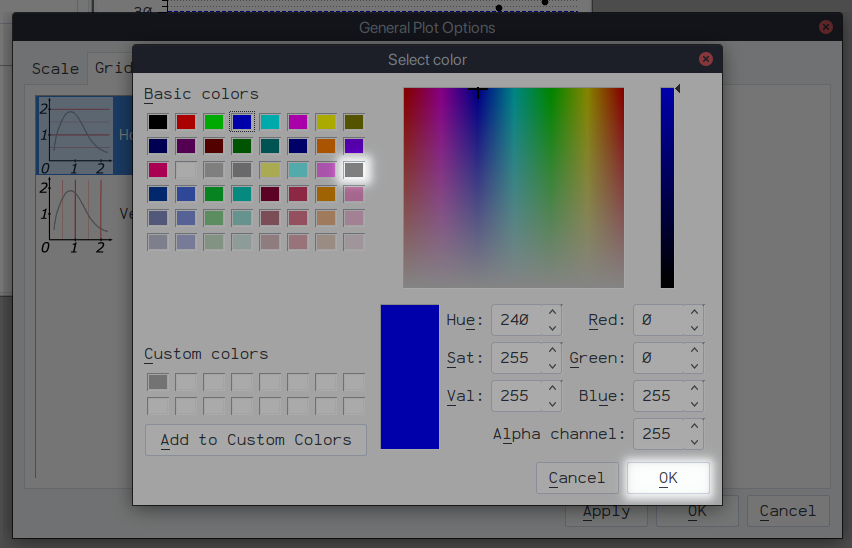
\includegraphics[width=\textwidth]{reta/6cor.png}

            \caption{Mudança de cor da linha}
            \label{fig:reta:gridcor}
        \end{subfigure}
        \caption{Opções de linhas de \textit{grid}}
        \label{fig:reta:opcoes_eixo}
    \end{figure}


\subsection{Resultado}

    \begin{figure}[htbp]
        \centering
        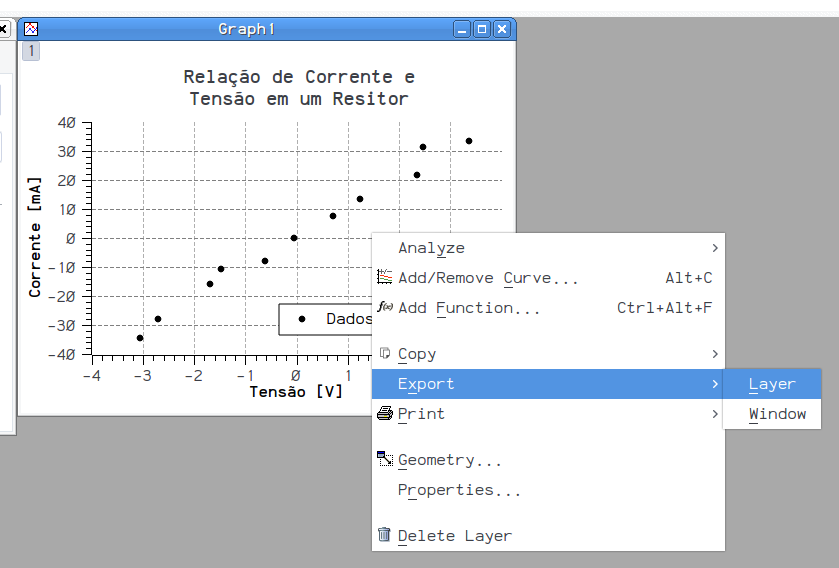
\includegraphics[width=0.6\textwidth]{reta/7save.png}

        \caption{Salvando o gráfico resultante}
        \label{fig:reta:salvar}
    \end{figure}

    \begin{figure}[htbp]
        \centering
        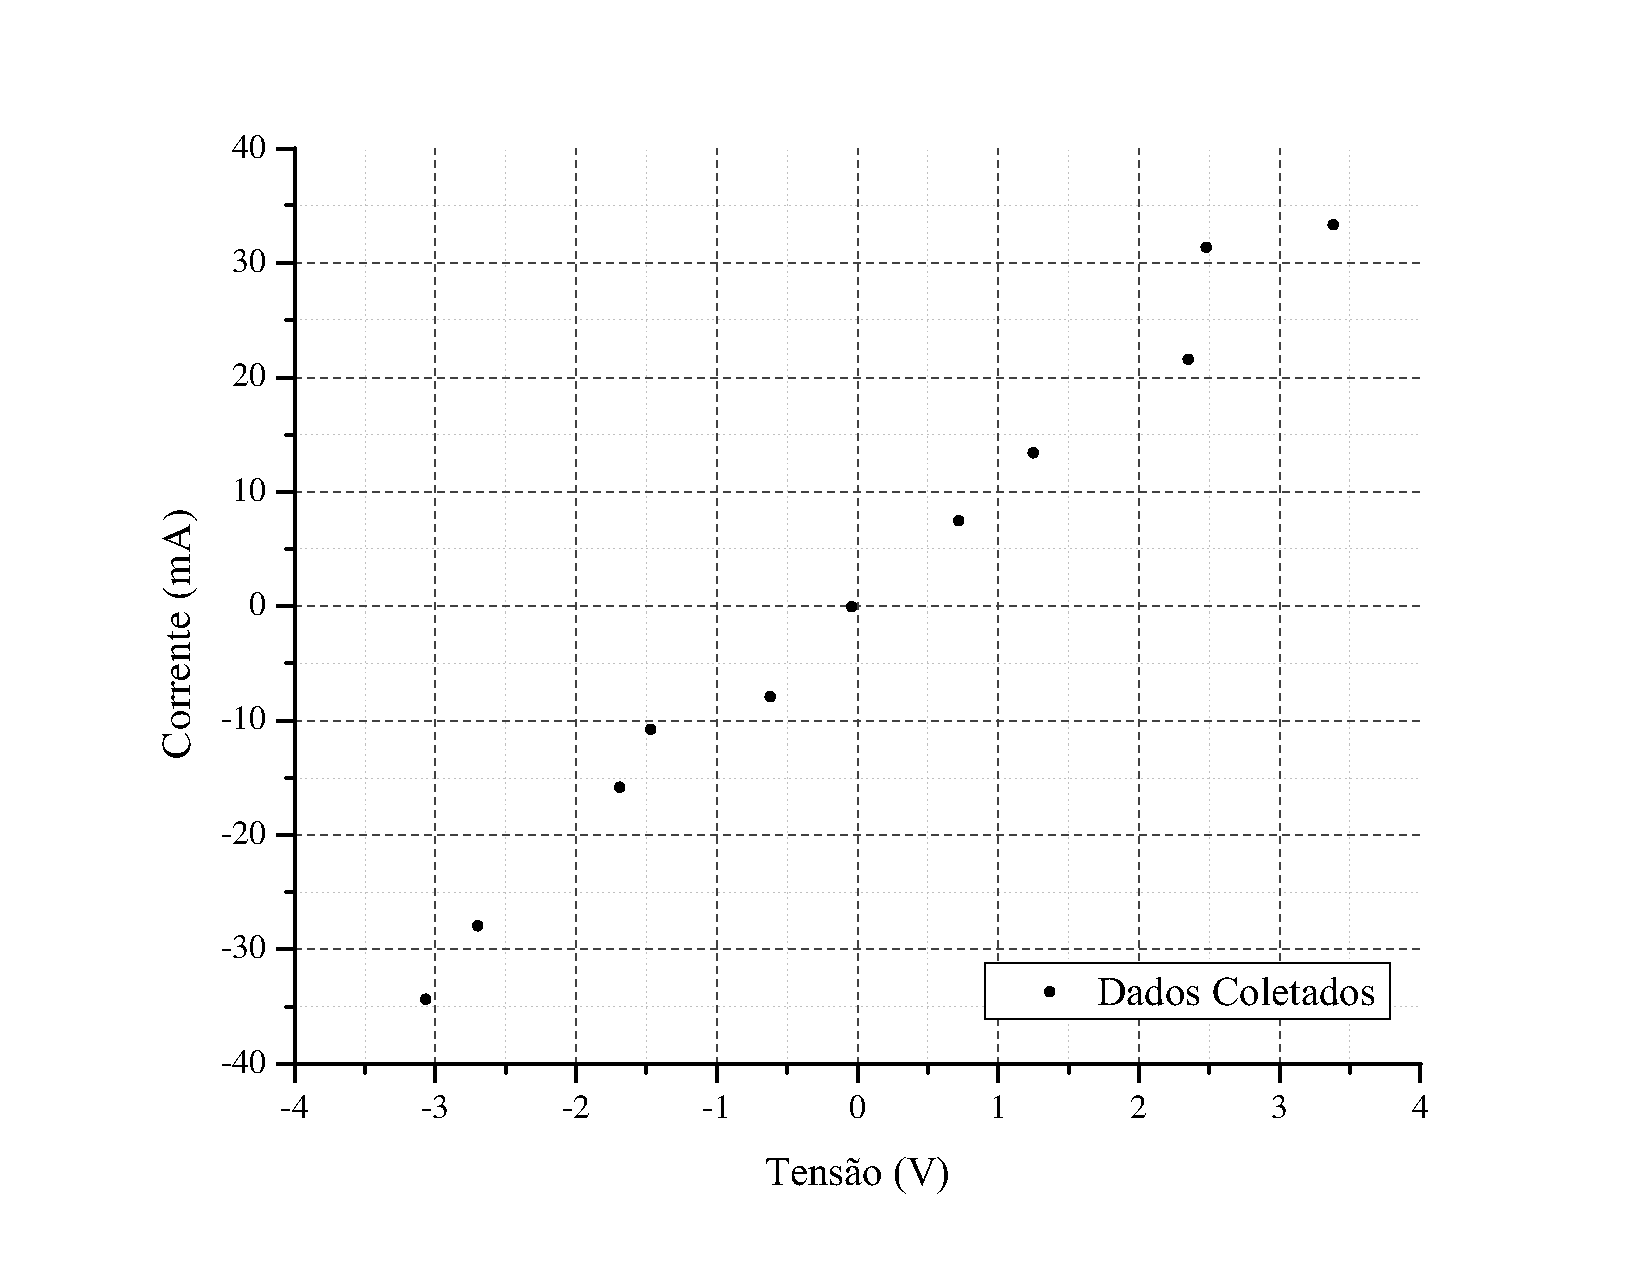
\includegraphics[width=0.6\textwidth]{reta/2gridlinscat.pdf}

        \caption{Gráfico de exemplo de formatação}
        \label{fig:reta:gridlinscat}
    \end{figure}

